% Provenance (never printed): cycle 3 / 6e "La planete Terre, l'environnement
% et l'action humaine" (the Earth in the Solar System; conditions for life);
% see sources/book1/PROVENANCE.md. Book 1, grade 6, chapter 1.
\chapter{La Tierra, un planeta del sistema solar}\label{ch:g6:earth-a-planet}

Tres sondas robot han sido enviadas al espacio. Una tras otra, mandan a
casa una imagen, como una postal. La primera llega de Venus: una bola
pálida envuelta en \omterm{def:g4:clouds-rain-snow:cloud}{nubes} espesas, donde hace calor suficiente para fundir
el plomo y el aire aprieta el suelo con un peso aplastante. La segunda
llega de Marte: un \omterm{def:g5:weather-and-climate:desert}{desierto} rojo, frío y polvoriento bajo un cielo tenue.
La tercera sonda ha vuelto su cámara hacia casa: una bola azul y blanca,
con \omterm{def:g2:water-on-earth:ocean}{océanos}, \omterm{def:g4:clouds-rain-snow:cloud}{nubes} y hielo. Tres planetas, vecinos alrededor del mismo Sol.
¿Por qué solo uno de ellos es azul?
% ledger: nasa:venus-clouds, nasa:mars-water

\begin{omfigure}
\begin{minipage}[t]{0.31\linewidth}\centering
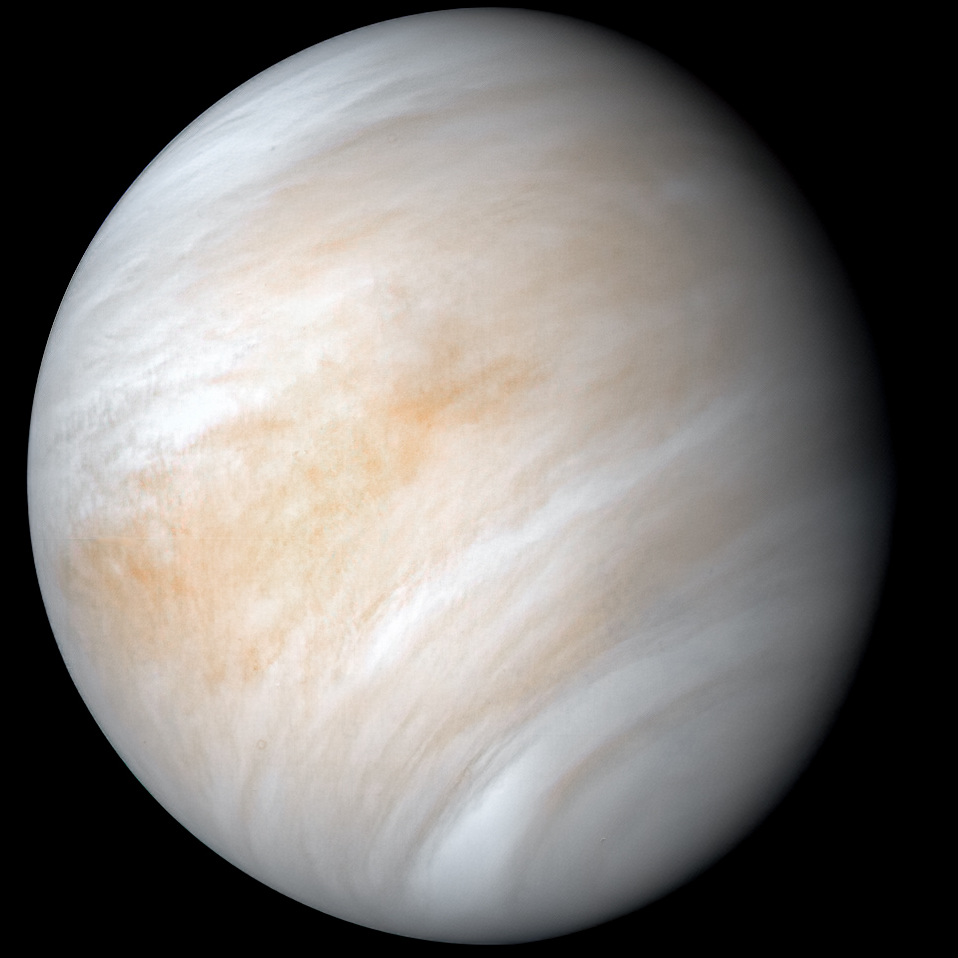
\includegraphics[width=\linewidth]{images/book1/g6-venus-mariner10.jpg}\\[2pt]
{\small Venus}
\end{minipage}\hfill
\begin{minipage}[t]{0.31\linewidth}\centering
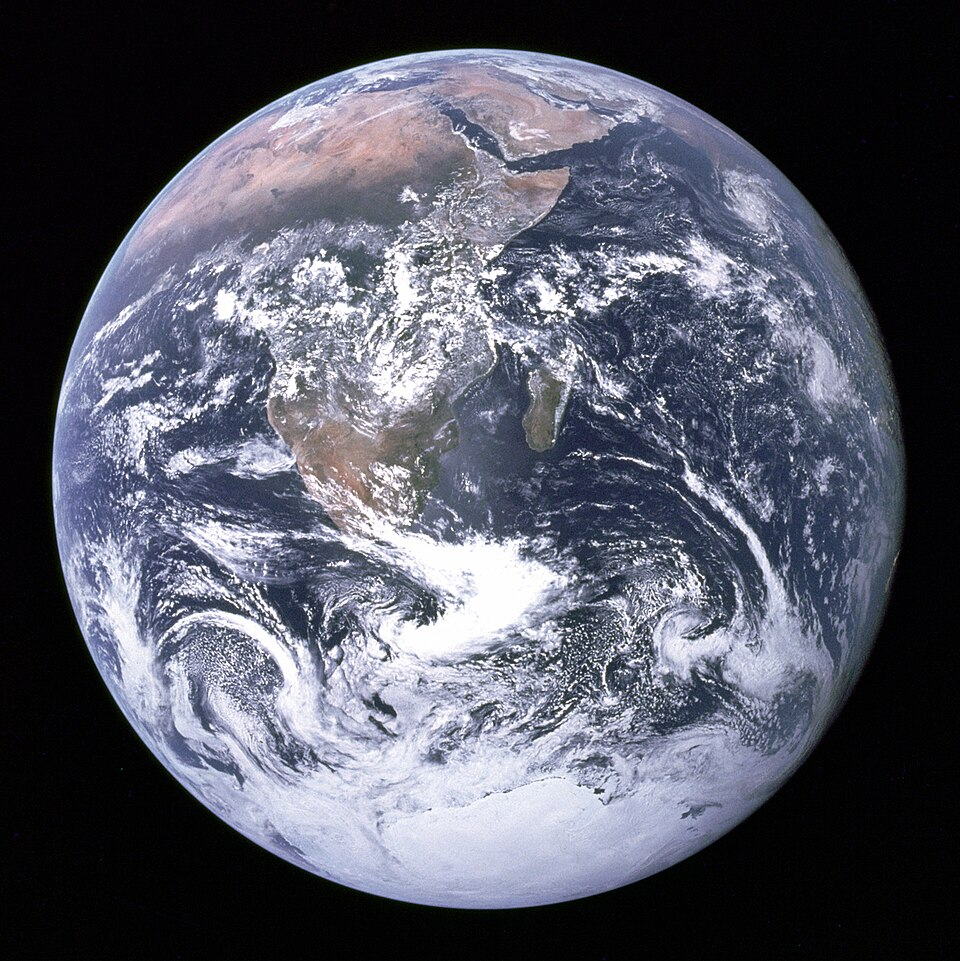
\includegraphics[width=\linewidth]{images/book1/g6-earth-apollo17.jpg}\\[2pt]
{\small La Tierra}
\end{minipage}\hfill
\begin{minipage}[t]{0.31\linewidth}\centering
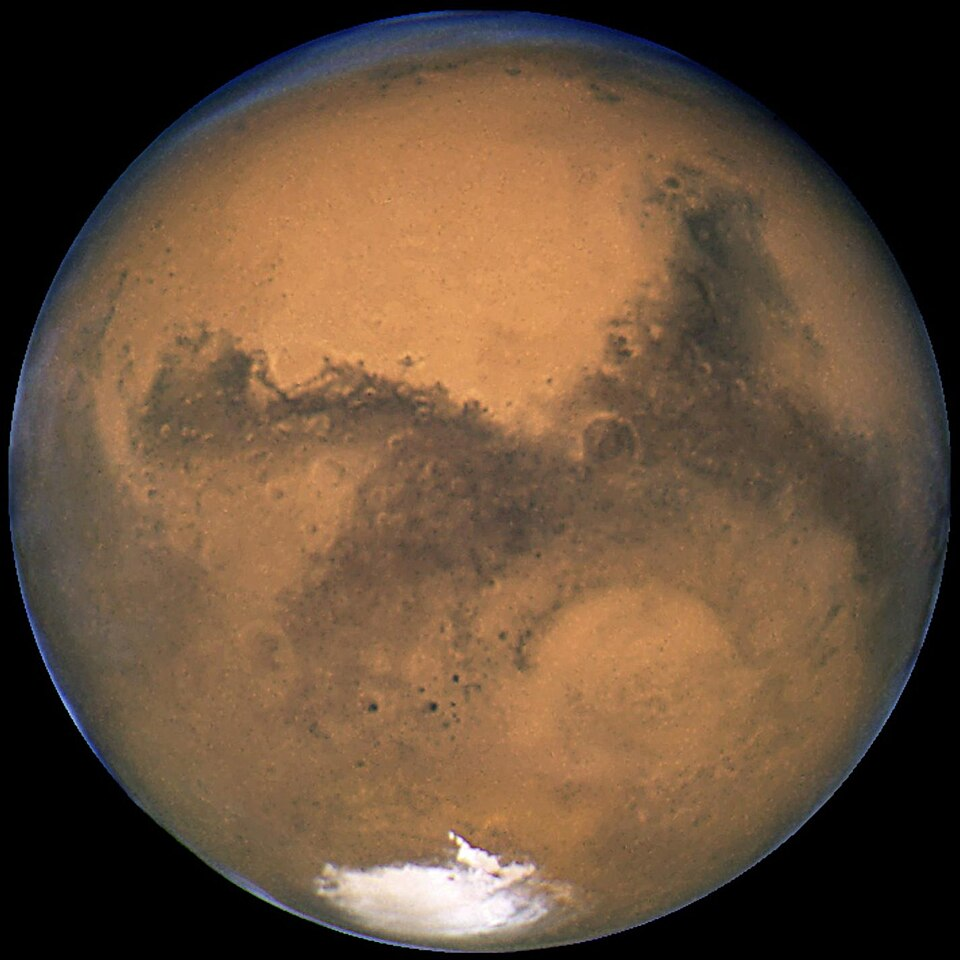
\includegraphics[width=\linewidth]{images/book1/g6-mars-hubble.jpg}\\[2pt]
{\small Marte}
\end{minipage}

\medskip
{\small Tres postales desde el espacio. Venus, fotografiado por la sonda
Mariner~10 en 1974: solo vemos la parte de arriba de sus \omterm{def:g4:clouds-rain-snow:cloud}{nubes}. La Tierra,
fotografiada por la tripulación del Apolo~17 de camino a la Luna en 1972:
África, Arabia y el hielo de la Antártida bajo \omterm{def:g4:clouds-rain-snow:cloud}{nubes} blancas. Marte,
fotografiado por el telescopio espacial Hubble en 2003, con un casquete
blanco de hielo en su \omterm{def:g3:continents-and-oceans:poles}{polo}. (Fotos: NASA/JPL-Caltech; NASA; NASA, ESA y
Hubble Heritage Team.)}
% ledger: nasa:venus-mariner10, nasa:apollo17-earth, hubble:mars-2003
\end{omfigure}

\begin{recall}
Los libros de física mostraron que el Sol es una estrella, una enorme bola
de gas caliente que brilla por sí misma, y que un planeta es un cuerpo
grande y redondo que gira alrededor de una estrella y no brilla por sí
mismo: lo vemos porque refleja la luz de su estrella. El Sol y todo lo que
gira a su alrededor forman el sistema solar. Cada planeta recorre alrededor
del Sol un camino llamado su órbita, y gira sobre sí mismo alrededor de un
eje. El aire que nos rodea aprieta todo lo que toca: es la presión del
aire. La densidad de un material indica cuánto pesa un volumen dado de él:
un centímetro cúbico de agua pesa 1~gramo, así que su densidad es de
1~gramo por centímetro cúbico; un material más denso que el agua se hunde
en ella, y uno menos denso flota. Por último, unas siete décimas partes de
la superficie de la Tierra están cubiertas por el \omterm{def:g2:water-on-earth:ocean}{océano}
(\cref{ch:g2:water-on-earth}).
\end{recall}

\section{Ocho planetas alrededor del Sol}

Ocho planetas giran alrededor del Sol. En orden, del más cercano al más
lejano, son Mercurio, Venus, la Tierra, Marte, Júpiter, Saturno, Urano y
Neptuno. Una frase puede ayudar a recordar el orden: \emph{Mi Viejo Tío
Mario Jamás Supo Usar Navaja} (Mercurio, Venus, Tierra, Marte, Júpiter,
Saturno, Urano, Neptuno).

El dibujo de abajo muestra los ocho planetas uno al lado del otro,
dibujados a la misma escala: si un planeta es el doble de ancho que otro,
su círculo también es el doble de ancho.

\begin{omfigure}
\pgfplotstableread{figdata/out/grade-6-planets-sizes.dat}\gsixsizes
\begin{tikzpicture}
  \draw[black!40] (-0.2,0) -- (13.8,0);
  \pgfplotstablegetrowsof{\gsixsizes}
  \pgfmathtruncatemacro{\gsixlast}{\pgfplotsretval-1}
  \foreach \i in {0,...,\gsixlast}{
    \pgfplotstablegetelem{\i}{x_cm}\of\gsixsizes \let\gx\pgfplotsretval
    \pgfplotstablegetelem{\i}{d_cm}\of\gsixsizes \let\gd\pgfplotsretval
    \def\gn{\ifcase\i Mercurio\or Venus\or Tierra\or Marte\or Júpiter\or Saturno\or Urano\or Neptuno\fi}%
    \pgfplotstablegetelem{\i}{d_km}\of\gsixsizes \let\gk\pgfplotsretval
    \pgfmathsetmacro{\gr}{\gd/2}
    \ifnum\i<4
      \fill[brown!70!black, draw=black!60, line width=0.3pt] (\gx,\gr) circle (\gr);
    \else
      \fill[orange!35, draw=black!60, line width=0.3pt] (\gx,\gr) circle (\gr);
    \fi
    \node[font=\scriptsize, rotate=40, anchor=north east, inner sep=1pt]
      at (\gx+0.08,-0.08) {\gn};
  }
  \node[font=\scriptsize, align=left, anchor=north west] at (-0.2,4.15)
    {\tikz\fill[brown!70!black, draw=black!60] (0,0) circle (2.2pt); planetas rocosos\\
     \tikz\fill[orange!35, draw=black!60] (0,0) circle (2.2pt); planetas gigantes};
  \draw[|-|, black!70] (0,2.2) -- (1,2.2)
    node[midway, above, font=\scriptsize] {35\,000 km};
\end{tikzpicture}

{\small Los ocho planetas dibujados a escala (diámetros de la ficha de
datos planetarios de la NASA). Las distancias entre ellos no están a
escala: son demasiado grandes para caber en ninguna página.}
% ledger: planet:Mercury.diameter, planet:Venus.diameter, planet:Earth.diameter, planet:Mars.diameter, planet:Jupiter.diameter, planet:Saturn.diameter, planet:Uranus.diameter, planet:Neptune.diameter (figdata/grade-6/planets.py, part sizes)
\end{omfigure}

Los cuatro planetas más cercanos al Sol son pequeños. Los cuatro siguientes
son gigantes: Júpiter es unas 11 veces más ancho que la Tierra. ¿Y el Sol?
Dibujado a la misma escala que los planetas de arriba, sería un disco de
unos 40~centímetros de diámetro, más ancho que esta página.
% ledger: planet:Jupiter.diameter, planet:Earth.diameter, sun:R (planets.py: sun_cm = 39.9 cm)

El tamaño no es la única diferencia. La tabla de abajo da, para cada
planeta, su diámetro, su densidad (en gramos por centímetro cúbico) y su
distancia al Sol.

\begin{center}
\small
\begin{tabular}{lrrrr}
\hline
planeta & diámetro (km) & densidad (g/cm$^3$) & distancia al Sol (millones de km)\\
\hline
Mercurio & 4\,879 & 5.4 & 58\\
Venus & 12\,104 & 5.2 & 108\\
Tierra & 12\,756 & 5.5 & 150\\
Marte & 6\,792 & 3.9 & 228\\
\hline
Júpiter & 142\,984 & 1.3 & 779\\
Saturno & 120\,536 & 0.7 & 1\,432\\
Urano & 51\,118 & 1.3 & 2\,867\\
Neptuno & 49\,528 & 1.6 & 4\,515\\
\hline
\end{tabular}
% ledger: planet:Mercury.diameter, planet:Venus.diameter, planet:Earth.diameter, planet:Mars.diameter, planet:Jupiter.diameter, planet:Saturn.diameter, planet:Uranus.diameter, planet:Neptune.diameter, planet:Mercury.density, planet:Venus.density, planet:Earth.density, planet:Mars.density, planet:Jupiter.density, planet:Saturn.density, planet:Uranus.density, planet:Neptune.density, planet:Mercury.dist, planet:Venus.dist, planet:Earth.dist, planet:Mars.dist, planet:Jupiter.dist, planet:Saturn.dist, planet:Uranus.dist, planet:Neptune.dist (figdata/grade-6/planets.py, main table)
\end{center}

Las densidades dividen los planetas en dos familias, sin nada entre ambas:
los cuatro primeros son densos, de más de 3.9~gramos por centímetro cúbico,
como la \omterm{def:g3:stones-pebbles-sand:rock}{roca} y el metal; los cuatro últimos son ligeros, de menos de
1.7~gramos por centímetro cúbico.

\begin{definition}[Planetas rocosos y planetas gigantes]\label{def:g6:earth-a-planet:planet-types}
Un \emph{planeta rocoso}\index{planeta rocoso} es un planeta pequeño y
denso, hecho de \omterm{def:g3:stones-pebbles-sand:rock}{roca} y metal, con una superficie sólida en la que puede
posarse una sonda: Mercurio, Venus, la Tierra y Marte. Un \emph{planeta
gigante}\index{planeta gigante} es un planeta muy grande y de densidad
baja, hecho sobre todo de gases y líquidos, sin una superficie sólida en
la que posarse: Júpiter, Saturno, Urano y Neptuno.
% ledger: nasa:planet-families
\end{definition}

\begin{omfigure}
\begin{minipage}[c]{0.6\linewidth}\centering
\begin{tikzpicture}
  \begin{axis}[ybar, bar width=11pt, width=\linewidth, height=5.4cm,
      ymin=0, ymax=6.2, xmin=-0.6, xmax=7.6,
      xtick={0,...,7}, xticklabels={Mercurio,Venus,Tierra,Marte,Júpiter,Saturno,Urano,Neptuno},
      xticklabel style={rotate=40, anchor=north east, font=\scriptsize},
      ytick={0,1,...,6}, ylabel={densidad (g/cm$^3$)},
      tick label style={font=\scriptsize}, label style={font=\scriptsize},
      axis x line*=bottom, axis y line*=left]
    \addplot[fill=brown!70!black, draw=black!60, bar shift=0pt, restrict x to domain=0:3]
      table[x=idx, y=density_gcm3] {figdata/out/grade-6-planets-density.dat};
    \addplot[fill=orange!35, draw=black!60, bar shift=0pt, restrict x to domain=4:7]
      table[x=idx, y=density_gcm3] {figdata/out/grade-6-planets-density.dat};
    \draw[blue!60!black, densely dashed] (axis cs:-0.6,1) -- (axis cs:7.6,1);
    \node[font=\scriptsize, blue!60!black, anchor=south, inner sep=1pt]
      at (axis cs:5,1) {agua};
  \end{axis}
\end{tikzpicture}
\end{minipage}\hfill
\begin{minipage}[c]{0.36\linewidth}\centering
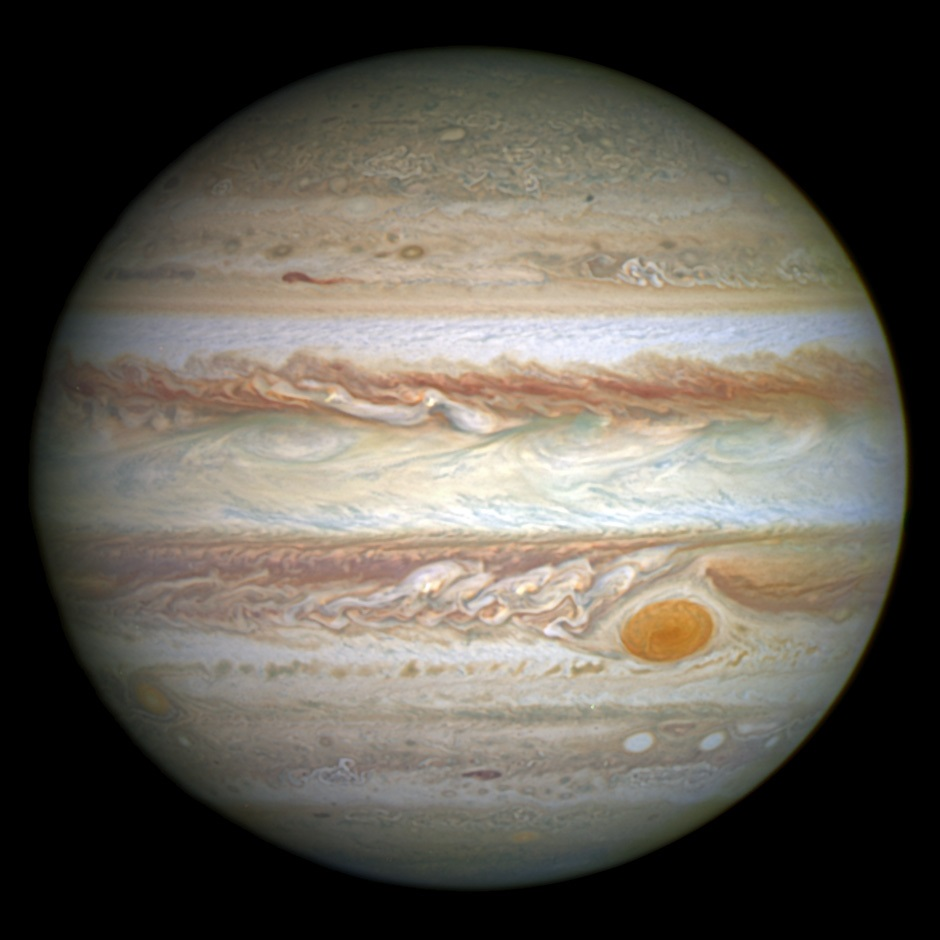
\includegraphics[width=0.9\linewidth]{images/book1/g6-jupiter-hubble.jpg}\\[2pt]
{\small Júpiter, fotografiado por el telescopio espacial Hubble en 2014.
(Foto: NASA, ESA, A.~Simon.)}
% ledger: hubble:jupiter-2014
\end{minipage}

\smallskip
{\small A la izquierda, la densidad de los ocho planetas; la línea
discontinua es la densidad del agua. A la derecha, lo que vemos de un
\omterm{def:g6:earth-a-planet:planet-types}{planeta gigante} es la parte de arriba de sus \omterm{def:g4:clouds-rain-snow:cloud}{nubes}.}
% ledger: planet:Mercury.density, planet:Venus.density, planet:Earth.density, planet:Mars.density, planet:Jupiter.density, planet:Saturn.density, planet:Uranus.density, planet:Neptune.density (figdata/grade-6/planets.py, part density)
\end{omfigure}

La fotografía de Júpiter muestra bandas de \omterm{def:g4:clouds-rain-snow:cloud}{nubes}, claras y oscuras, y un
óvalo rojo: la Gran Mancha Roja, una \omterm{def:g5:natural-hazards:storm}{tormenta} gigante más grande que toda
la Tierra, que lleva cientos de años soplando. Bajo las \omterm{def:g4:clouds-rain-snow:cloud}{nubes} no hay
suelo: solo gases, sobre todo hidrógeno y helio, cada vez más densos a
medida que se baja.
% ledger: nasa:jupiter-gas

\begin{remark}[Un planeta más ligero que el agua]\label{rem:g6:earth-a-planet:saturn}
Saturno es el único planeta cuya densidad es menor que la del agua: unos
0.7~gramos por centímetro cúbico. Si hubiera una bañera lo bastante grande
para meterlo, ¡Saturno flotaría!
% ledger: nasa:saturn-float, planet:Saturn.density
\end{remark}

\section{¿A qué distancia están los planetas?}

Los planetas no solo tienen tamaños muy distintos; también están muy
lejos unos de otros. La Tierra está a unos 150~millones de kilómetros del
Sol. Neptuno, el planeta más lejano, está 30~veces más lejos: a unos
4500~millones de kilómetros. El dibujo de abajo pone los ocho planetas en
una línea, a sus distancias del Sol, a escala.
% ledger: planet:Earth.dist, planet:Neptune.dist

\begin{omfigure}
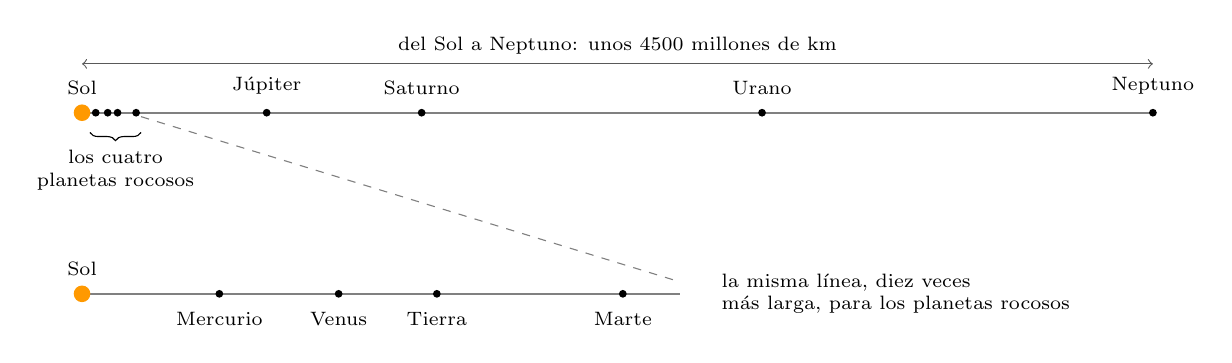
\begin{tikzpicture}
  % whole system
  \draw[thick, gray] (0,0) -- (13.6,0);
  \fill[orange!80!yellow] (0,0) circle (3pt);
  \node[font=\scriptsize, above=3pt] at (0,0) {Sol};
  \foreach \n/\x/\lab in {Mercurio/0.174/, Venus/0.326/, Tierra/0.451/, Marte/0.687/,
                          Júpiter/2.345/Júpiter, Saturno/4.313/Saturno, Urano/8.636/Urano, Neptuno/13.6/Neptuno} {
    \fill (\x,0) circle (1.4pt);
    \node[font=\scriptsize, above=3pt] at (\x,0) {\lab};
  }
  \draw[decorate, decoration={brace, amplitude=3pt, mirror}] (0.1,-0.25) -- (0.75,-0.25)
    node[midway, below=3pt, font=\scriptsize, align=center] {los cuatro\\ planetas rocosos};
  \draw[<->, thin, gray!70!black] (0,0.62) -- (13.6,0.62) node[midway, above, font=\scriptsize, black] {del Sol a Neptuno: unos 4500 millones de km};
  % the inner system, ten times larger
  \begin{scope}[yshift=-2.3cm]
    \draw[thick, gray] (0,0) -- (7.6,0);
    \fill[orange!80!yellow] (0,0) circle (3pt);
    \node[font=\scriptsize, above=3pt] at (0,0) {Sol};
    \foreach \n/\x in {Mercurio/1.744, Venus/3.259, Tierra/4.506, Marte/6.868} {
      \fill (\x,0) circle (1.4pt);
      \node[font=\scriptsize, below=3pt] at (\x,0) {\n};
    }
    \node[font=\scriptsize, anchor=west, align=left] at (8.0,0) {la misma línea, diez veces\\ más larga, para los planetas rocosos};
  \end{scope}
  \draw[dashed, gray] (0.75,-0.05) -- (7.6,-2.15);
\end{tikzpicture}

{\small Las distancias de los planetas al Sol, a escala. Arriba, todo el
sistema solar, del Sol a Neptuno. Abajo, los cuatro \omterm{def:g6:earth-a-planet:planet-types}{planetas rocosos},
ampliados diez veces. El tamaño de los puntos no está a escala.}
% ledger: planet:Mercury.dist, planet:Venus.dist, planet:Earth.dist, planet:Mars.dist, planet:Jupiter.dist, planet:Saturn.dist, planet:Uranus.dist, planet:Neptune.dist (figdata/grade-6/planets.py, part dist)
\end{omfigure}

Los cuatro \omterm{def:g6:earth-a-planet:planet-types}{planetas rocosos} están todos cerca del Sol; los cuatro \omterm{def:g6:earth-a-planet:planet-types}{planetas
gigantes} están muy lejos, con enormes huecos entre ellos. Solo el hueco entre Marte y Júpiter, de unos 550~millones de kilómetros, es más del doble de la distancia del Sol a Marte.
% ledger: planet:Mars.dist, planet:Jupiter.dist

Es difícil dibujar los tamaños y las distancias a la misma escala: los
planetas se convierten en puntos invisibles. Una \emph{maqueta a escala}
ayuda a imaginar las dos cosas a la vez.

\begin{method}[Construir una maqueta a escala del sistema solar]\label{met:g6:earth-a-planet:scale-model}
\begin{enumerate}
  \item Elige el tamaño de la Tierra en la maqueta, por ejemplo 1~cm.
  \item Calcula cuántos kilómetros reales representa 1~cm de la maqueta:
        divide el diámetro real de la Tierra (12\,756~km) entre su tamaño en
        la maqueta.
  \item Divide cada tamaño real y cada distancia real entre ese número.
        Después cambia las unidades por otras fáciles de imaginar
        (centímetros, metros, kilómetros).
\end{enumerate}
% ledger: planet:Earth.diameter
\end{method}

\begin{example}[Una canica como Tierra]\label{ex:g6:earth-a-planet:marble}
Si la Tierra es una canica de 1~cm de ancho, 1~cm representa 12\,756~km.
El Sol, de 1\,391\,400~km de diámetro, se convierte en una bola de
$1\,391\,400 \div 12\,756 \approx
109$~cm de ancho: una bola más alta que un niño pequeño. La Tierra está a
150~millones de~km del Sol: $149\,600\,000 \div 12\,756 \approx 11\,700$~cm,
es decir, unos 117~metros, la longitud de un campo de fútbol.
% ledger: planet:Earth.diameter, sun:R, planet:Earth.dist
\end{example}

\begin{center}\small
\begin{tabular}{|l|c|c|}
\hline
\textbf{cuerpo} & \textbf{tamaño en la maqueta (cm)} & \textbf{distancia al Sol (m)} \\
\hline
el Sol & 109 & --- \\
Mercurio & 0.38 & 45 \\
Venus & 0.95 & 85 \\
la Tierra & 1.00 & 117 \\
Marte & 0.53 & 179 \\
Júpiter & 11.21 & 610 \\
Saturno & 9.45 & 1123 \\
Urano & 4.01 & 2248 \\
Neptuno & 3.88 & 3540 \\
\hline
\end{tabular}
\end{center}
% ledger: sun:R, planet:Mercury.diameter, planet:Venus.diameter, planet:Earth.diameter, planet:Mars.diameter, planet:Jupiter.diameter, planet:Saturn.diameter, planet:Uranus.diameter, planet:Neptune.diameter, planet:Mercury.dist, planet:Venus.dist, planet:Earth.dist, planet:Mars.dist, planet:Jupiter.dist, planet:Saturn.dist, planet:Uranus.dist, planet:Neptune.dist (figdata/grade-6/planets.py, part model)

En esta maqueta, todo el sistema solar hasta Neptuno se extiende sobre un
círculo de 7~km de diámetro, con una bola grande en el centro y ocho
canicas y bolas, la mayor del tamaño de un pomelo, repartidas por él. El
sistema solar es sobre todo espacio vacío.

\section{Venus, la Tierra y Marte}

Venus, la Tierra y Marte son vecinos, y los tres son \omterm{def:g6:earth-a-planet:planet-types}{planetas rocosos}.
Venus tiene casi el mismo tamaño que la Tierra: su diámetro es el 95~\% del
de la Tierra. Marte es más pequeño: su diámetro es más o menos la mitad del
de la Tierra. Y, sin embargo, estos tres planetas difícilmente podrían ser
más distintos.
% ledger: planet:Venus.diameter, planet:Earth.diameter, planet:Mars.diameter (planets.py: 94.9 %)

\paragraph{Venus.} Venus está envuelto en una capa espesa de aire, hecha
sobre todo de dióxido de carbono, con \omterm{def:g4:clouds-rain-snow:cloud}{nubes} densas de ácido sulfúrico, un
ácido que quema. Su aire es tan espeso que aprieta el suelo 92~veces más
fuerte de lo que el aire de la Tierra aprieta el nuestro. En la superficie,
la temperatura es de unos 464~$^\circ$C: calor suficiente para fundir el
plomo. Allí ningún agua puede seguir líquida.
% ledger: nasa:venus-clouds, planet:Venus.psurf, planet:Venus.Tmean

\paragraph{Marte.} Marte es un \omterm{def:g5:weather-and-climate:desert}{desierto} frío, seco y polvoriento. Su aire
también está hecho sobre todo de dióxido de carbono, pero es muy tenue:
aprieta el suelo unas cien veces menos que el aire de la Tierra. La
temperatura media es de $-65$~$^\circ$C. Hoy hay agua allí, pero helada:
en forma de hielo en los casquetes polares y bajo el suelo cerca de los
\omterm{def:g3:continents-and-oceans:poles}{polos}. Sin embargo, Marte no siempre fue así: hace miles de millones de
años, por Marte corrían \omterm{def:g1:landscapes-around-us:water}{ríos}, se formaban \omterm{def:g1:landscapes-around-us:water}{lagos} y pasaban \omterm{def:g5:water-shapes-the-land:flood}{inundaciones}.
% ledger: nasa:mars-water, planet:Mars.psurf, planet:Mars.Tmean

\paragraph{La Tierra.} Entre los dos, la Tierra tiene un aire que aprieta
el suelo con alrededor de 1~bar (la unidad que se usa para comparar la
presión del aire en los planetas), una temperatura media de 15~$^\circ$C y
\omterm{def:g2:water-on-earth:ocean}{océanos} de agua líquida.
% ledger: planet:Earth.psurf, planet:Earth.Tmean

\begin{omfigure}
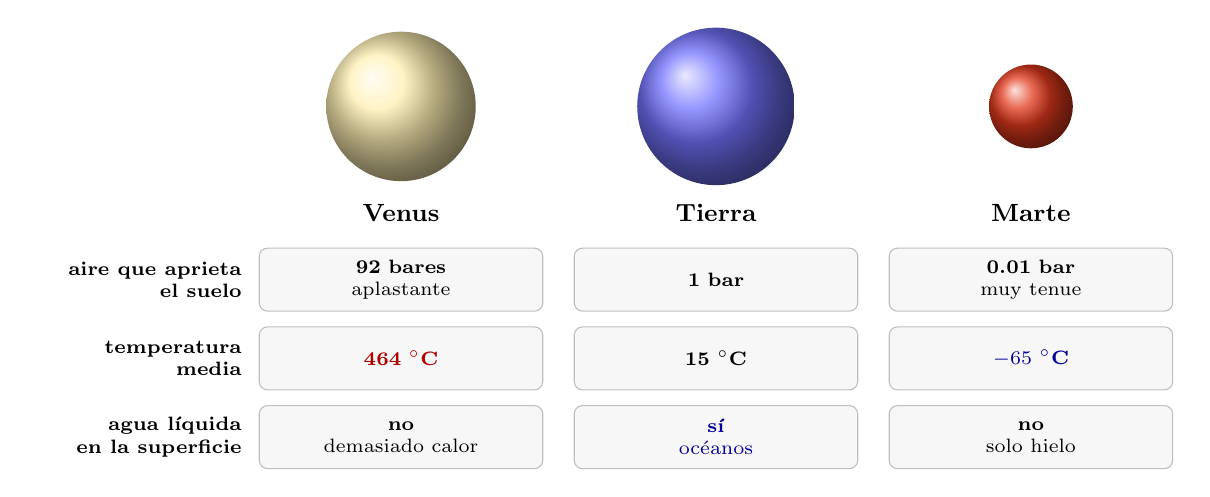
\begin{tikzpicture}[x=1cm, y=1cm,
    lab/.style={font=\scriptsize, align=center, text width=3.6cm},
    row/.style={font=\scriptsize\bfseries, anchor=east, align=right, text width=2.6cm}]
  % discs to scale: diameters 94.9 %, 100 %, 53.2 % of the Earth's (planets.py)
  \shade[ball color=yellow!60!orange!30] (3,0) circle (0.949);
  \shade[ball color=blue!55] (7,0) circle (1.0);
  \shade[ball color=red!55!brown] (11,0) circle (0.532);
  \node[font=\small\bfseries] at (3,-1.35) {Venus};
  \node[font=\small\bfseries] at (7,-1.35) {Tierra};
  \node[font=\small\bfseries] at (11,-1.35) {Marte};
  \foreach \y/\t in {-2.2/{aire que aprieta\\el suelo}, -3.2/{temperatura\\media},
                     -4.2/{agua líquida\\en la superficie}}
    {\node[row] at (1.1,\y) {\t};}
  \foreach \x in {3,7,11}{
    \foreach \y in {-2.2,-3.2,-4.2}{
      \draw[rounded corners=3pt, black!25, fill=black!3] (\x-1.8,\y-0.4) rectangle (\x+1.8,\y+0.4);}}
  \node[lab] at (3,-2.2) {\textbf{92 bares}\\aplastante};
  \node[lab] at (7,-2.2) {\textbf{1 bar}};
  \node[lab] at (11,-2.2) {\textbf{0.01 bar}\\muy tenue};
  \node[lab, text=red!70!black] at (3,-3.2) {\textbf{464~$^\circ$C}};
  \node[lab] at (7,-3.2) {\textbf{15~$^\circ$C}};
  \node[lab, text=blue!60!black] at (11,-3.2) {\textbf{$-65$~$^\circ$C}};
  \node[lab] at (3,-4.2) {\textbf{no}\\demasiado calor};
  \node[lab, text=blue!60!black] at (7,-4.2) {\textbf{sí}\\océanos};
  \node[lab] at (11,-4.2) {\textbf{no}\\solo hielo};
\end{tikzpicture}

{\small Venus, la Tierra y Marte comparados. Los tres discos están
dibujados a escala. (Valores: ficha de datos planetarios de la NASA.)}
% ledger: planet:Venus.psurf, planet:Earth.psurf, planet:Mars.psurf, planet:Mercury.Tmean, planet:Venus.Tmean, planet:Earth.Tmean, planet:Mars.Tmean, planet:Jupiter.Tmean, planet:Saturn.Tmean, planet:Uranus.Tmean, planet:Neptune.Tmean, nasa:mars-water
\end{omfigure}

\paragraph{Calor y frío.} Cerca del Sol, un planeta recibe mucha de su luz
y de su calor; lejos de él, muy poco. Así que cuanto más lejos del Sol está
un planeta, más frío debería ser. El gráfico de abajo muestra que es cierto
de la Tierra hacia fuera: los \omterm{def:g6:earth-a-planet:planet-types}{planetas gigantes}, muy lejanos, son mundos
helados. Pero fíjate en Venus: está casi el doble de lejos del Sol que
Mercurio, ¡y sin embargo es más caliente! Su aire espeso de dióxido de
carbono atrapa el calor del Sol como una manta gruesa y no lo deja
escapar. Mercurio, casi sin aire, no puede conservar su calor.
% ledger: planet:Mercury.Tmean, planet:Venus.Tmean, planet:Earth.Tmean, planet:Mars.Tmean, planet:Jupiter.Tmean, planet:Saturn.Tmean, planet:Uranus.Tmean, planet:Neptune.Tmean, planet:Mercury.dist, planet:Venus.dist, planet:Earth.dist, planet:Mars.dist, planet:Jupiter.dist, planet:Saturn.dist, planet:Uranus.dist, planet:Neptune.dist, nasa:venus-clouds, planet:Mercury.psurf

\begin{omfigure}
\begin{tikzpicture}
  \begin{axis}[ybar, bar width=14pt, width=0.86\linewidth, height=6cm,
      ymin=-270, ymax=520, xmin=-0.6, xmax=7.6,
      xtick={0,...,7},
      xticklabels={{Mercurio\\58}, {Venus\\108}, {Tierra\\150}, {Marte\\228},
                   {Júpiter\\779}, {Saturno\\1432}, {Urano\\2867}, {Neptuno\\4515}},
      xticklabel style={align=center, font=\scriptsize},
      axis x line*=bottom, axis y line*=left,
      xticklabel pos=lower, ytick={-200,-100,...,500},
      ylabel={temperatura media ($^\circ$C)}, xlabel={planeta y distancia al Sol (millones de km)},
      tick label style={font=\scriptsize}, label style={font=\scriptsize},
      nodes near coords, nodes near coords style={font=\tiny},
      every node near coord/.append style={/pgf/number format/1000 sep={}}]
    \addplot[fill=orange!50, draw=black!60, bar shift=0pt]
      table[x=idx, y=tmean_C] {figdata/out/grade-6-planets-temp.dat};
    \draw[black!50] (axis cs:-0.6,0) -- (axis cs:7.6,0);
  \end{axis}
\end{tikzpicture}

{\small La temperatura media de los planetas, en orden de distancia al Sol.
Venus rompe la regla: es más caliente que Mercurio, que está más cerca del
Sol. (Valores: ficha de datos planetarios de la NASA.)}
% ledger: planet:Mercury.Tmean, planet:Venus.Tmean, planet:Earth.Tmean, planet:Mars.Tmean, planet:Jupiter.Tmean, planet:Saturn.Tmean, planet:Uranus.Tmean, planet:Neptune.Tmean, planet:Mercury.dist, planet:Venus.dist, planet:Earth.dist, planet:Mars.dist, planet:Jupiter.dist, planet:Saturn.dist, planet:Uranus.dist, planet:Neptune.dist (figdata/grade-6/planets.py, part temp)
\end{omfigure}

\section{Lo que hace posible la vida en la Tierra}

La Tierra es el único planeta en el que sabemos que existe la vida. Los
seres vivos necesitan varias condiciones a la vez, y la Tierra las tiene
todas.

\begin{itemize}
  \item \textbf{Agua líquida.} Todos los seres vivos necesitan agua
        líquida: la Tierra tiene \omterm{def:g2:water-on-earth:ocean}{océanos}, \omterm{def:g1:landscapes-around-us:water}{ríos} y \omterm{def:g1:landscapes-around-us:water}{lagos}.
  \item \textbf{Temperaturas suaves.} En la superficie de la Tierra, el
        agua se congela a 0~$^\circ$C y hierve a 100~$^\circ$C (física).
        Con una media de 15~$^\circ$C, las temperaturas de la Tierra se
        mantienen casi siempre entre las dos, así que su agua sigue líquida.
  \item \textbf{La distancia adecuada al Sol.} Más cerca del Sol, como
        Venus, un planeta corre el riesgo de ser demasiado caliente; más
        lejos, como Marte, demasiado frío. La Tierra está a la distancia
        adecuada para tener agua líquida.
  \item \textbf{Una atmósfera.} La capa de aire que rodea la Tierra mantiene
        caliente su superficie por la noche, da a los seres vivos los gases
        que necesitan y aprieta lo suficiente sobre los \omterm{def:g2:water-on-earth:ocean}{océanos} para que su
        agua siga líquida. En Marte, el aire es tan tenue que el agua
        líquida no puede durar mucho en la superficie: se congela o se
        convierte en vapor.
\end{itemize}
% ledger: nasa:mars-water, planet:Earth.Tmean

\begin{remark}[¿Hubo vida en Marte?]\label{rem:g6:earth-a-planet:mars-life}
Como Marte tuvo en otro tiempo \omterm{def:g1:landscapes-around-us:water}{ríos} y \omterm{def:g1:landscapes-around-us:water}{lagos}, los científicos se preguntan
si pudieron vivir allí seres vivos diminutos, hace mucho, cuando Marte era
más cálido y húmedo. Los científicos no esperan encontrar seres vivos en
Marte hoy; con robots exploradores, buscan en sus \omterm{def:g3:stones-pebbles-sand:rock}{rocas} señales de una vida
que existió hace mucho tiempo.
% ledger: nasa:mars-water
\end{remark}

\section{La Tierra vista desde el espacio}

Durante miles de años, la gente solo podía imaginar cómo era su planeta
visto desde fuera. El 24~de~diciembre~de~1968, los astronautas del Apolo~8,
en órbita alrededor de la Luna, vieron salir la Tierra sobre el horizonte
gris de la Luna, y uno de ellos, Bill Anders, tomó la fotografía de abajo.
% ledger: nasa:earthrise

\begin{omfigure}
\begin{minipage}[c]{0.46\linewidth}\centering
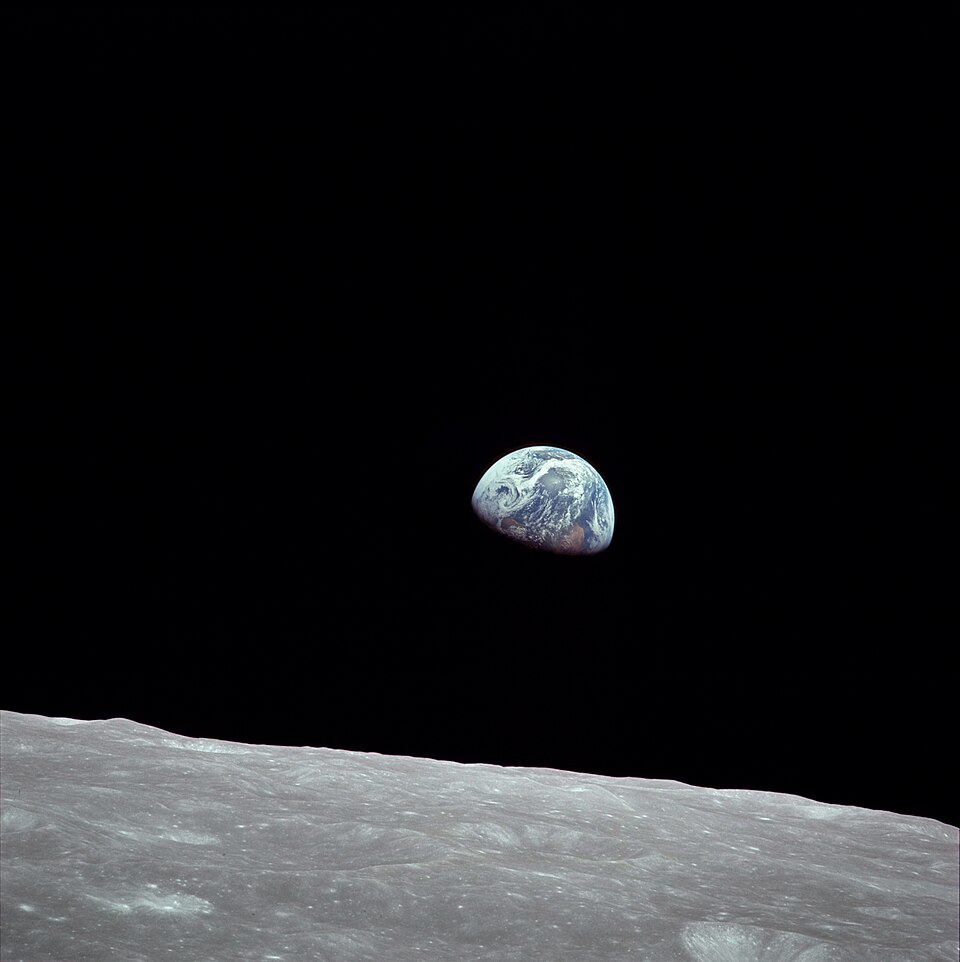
\includegraphics[width=0.85\linewidth]{images/book1/g6-earthrise.jpg}
\end{minipage}\hfill
\begin{minipage}[c]{0.5\linewidth}
{\small \emph{Salida de la Tierra}: la Tierra sobre el horizonte de la Luna,
fotografiada desde el Apolo~8 en órbita alrededor de la Luna,
el 24~de~diciembre~de~1968. (Foto: NASA, Bill Anders.)}

\medskip
{\small Fíjate en los colores: el azul de los \omterm{def:g2:water-on-earth:ocean}{océanos}, los remolinos blancos
de las \omterm{def:g4:clouds-rain-snow:cloud}{nubes}, el marrón de la tierra firme. Alrededor, el negro del
espacio; en primer plano, el suelo gris y muerto de la Luna, sin agua y sin
aire.}
\end{minipage}
% ledger: nasa:earthrise
\end{omfigure}

Vista desde el espacio, la Tierra es sobre todo azul: el \omterm{def:g2:water-on-earth:ocean}{océano} cubre unas
siete décimas partes de su superficie. Por encima giran \omterm{def:g4:clouds-rain-snow:cloud}{nubes} blancas de
gotitas de agua, y un hielo blanco cubre los \omterm{def:g3:continents-and-oceans:poles}{polos}. La tierra firme es
marrón donde está seca y verde donde crecen plantas. El propio aire no se
ve, pero las \omterm{def:g4:clouds-rain-snow:cloud}{nubes} que flotan en él muestran que está ahí. De todos los planetas del sistema solar, solo la Tierra muestra estos colores
juntos: agua líquida, \omterm{def:g4:clouds-rain-snow:cloud}{nubes} y plantas vivas.
% ledger: wss:ocean-cover, nasa:apollo17-earth

\begin{history}[El punto azul pálido]
\begin{minipage}[c]{0.66\linewidth}
El 14~de~febrero~de~1990, la sonda espacial Voyager~1 estaba a unos
6\,000~millones de kilómetros del Sol, más lejos que Neptuno. Antes de
dejar atrás el sistema solar, volvió su cámara y tomó una imagen de la
Tierra. En la fotografía, nuestro planeta es una sola mota brillante, más
pequeña que un grano de polvo, atrapada en un rayo de luz del Sol. El
astrónomo Carl Sagan escribió sobre ella: ``Mira otra vez ese punto. Eso es
aquí. Eso es nuestro hogar. Eso somos nosotros''.
% ledger: nasa:pale-blue-dot
\end{minipage}\hfill
\begin{minipage}[c]{0.3\linewidth}\centering
\begin{tikzpicture}
  \node[inner sep=0] (img) {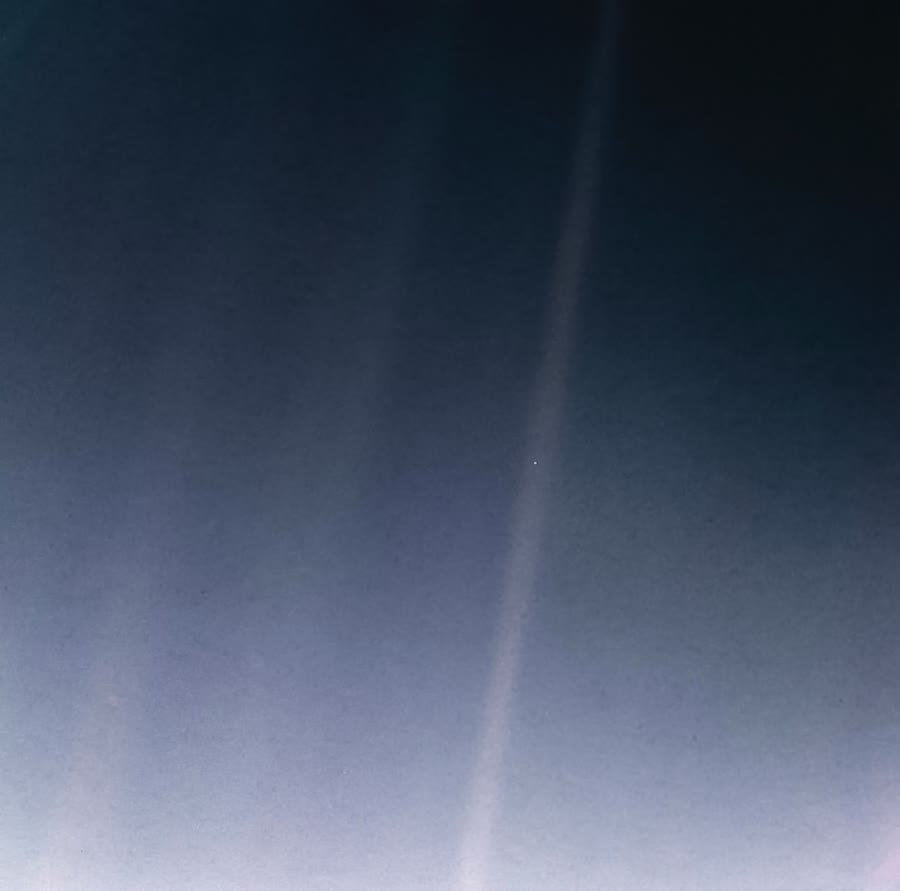
\includegraphics[width=\linewidth]{images/book1/g6-pale-blue-dot.jpg}};
  \draw[yellow!80!orange, thick] ($(img.south west)!0.594!(img.south east) + (0,{0.476*\linewidth})$) circle (6pt);
\end{tikzpicture}\\[2pt]
{\footnotesize La Tierra (en el círculo) vista por la Voyager~1, 1990.
(Imagen: NASA/JPL-Caltech, dominio público.)}
% ledger: nasa:pale-blue-dot
\end{minipage}
\end{history}

\section{Ejercicios}

\begin{exercise}[$\star$]\label{exo:g6:earth-a-planet:1}
Escribe en orden los ocho planetas del sistema solar, del más cercano al
Sol al más lejano. Subraya los \omterm{def:g6:earth-a-planet:planet-types}{planetas rocosos}.
\end{exercise}

\begin{exercise}[$\star$]\label{exo:g6:earth-a-planet:2}
Copia y completa: ``Un \omterm{def:g6:earth-a-planet:planet-types}{planeta rocoso} es pequeño y \ldots, con una
superficie \ldots{} Un \omterm{def:g6:earth-a-planet:planet-types}{planeta gigante} es muy grande, de \ldots{} baja,
hecho sobre todo de \ldots{} y de \ldots{}''
\end{exercise}

\begin{exercise}[$\star$]\label{exo:g6:earth-a-planet:3}
Según la tabla de este capítulo, ¿qué planeta tiene el diámetro más
parecido al de la Tierra? ¿Cuál es el planeta más grande? ¿Cuál es el más
pequeño?
\end{exercise}

\begin{exercise}[$\star$]\label{exo:g6:earth-a-planet:4}
¿Verdadero o falso? Corrige las frases falsas.
(a) Venus está cubierto de \omterm{def:g2:water-on-earth:ocean}{océanos}.
(b) Marte es más frío que la Tierra.
(c) Los \omterm{def:g6:earth-a-planet:planet-types}{planetas gigantes} son los cuatro planetas más cercanos al Sol.
(d) Saturno es menos denso que el agua.
\end{exercise}

\begin{exercise}[$\star\star$]\label{exo:g6:earth-a-planet:5}
El diámetro de Mercurio es de 4\,879~km, y el de la Tierra, de
12\,756~km. Calcula el diámetro de Mercurio como porcentaje del de la
Tierra, redondeado al número entero más cercano.
% ledger: planet:Mercury.diameter, planet:Earth.diameter (planets.py: 38.2 %)
\end{exercise}

\begin{exercise}[$\star\star$]\label{exo:g6:earth-a-planet:6}
¿Cuántas Tierras, una al lado de otra, cabrían en el diámetro de Saturno
(120\,536~km)? Redondea al número entero más cercano. ¿Saturno es un
\omterm{def:g6:earth-a-planet:planet-types}{planeta rocoso} o un \omterm{def:g6:earth-a-planet:planet-types}{planeta gigante}?
% ledger: planet:Saturn.diameter, planet:Earth.diameter
\end{exercise}

\begin{exercise}[$\star\star$]\label{exo:g6:earth-a-planet:7}
Los astrónomos han encontrado planetas alrededor de otras estrellas. El
planeta~A tiene una densidad de 1.1~gramos por centímetro cúbico y es
9~veces más ancho que la Tierra. El planeta~B tiene una densidad de
5.0~gramos por centímetro cúbico y es un poco más pequeño que la Tierra.
¿Cuál es un \omterm{def:g6:earth-a-planet:planet-types}{planeta rocoso} y cuál un \omterm{def:g6:earth-a-planet:planet-types}{planeta gigante}? Explícalo.
\end{exercise}

\begin{exercise}[$\star\star$]\label{exo:g6:earth-a-planet:8}
Usa el gráfico de las temperaturas de los planetas: (a) ¿cuántos grados
más caliente que la Tierra es Venus? (b) ¿Cuántos grados más frío que la
Tierra es Marte?
% ledger: planet:Venus.Tmean, planet:Earth.Tmean, planet:Mars.Tmean
\end{exercise}

\begin{exercise}[$\star\star$]\label{exo:g6:earth-a-planet:9}
Mercurio es el planeta más cercano al Sol, pero Venus es el más caliente.
Explica por qué.
\end{exercise}

\begin{exercise}[$\star\star$]\label{exo:g6:earth-a-planet:10}
La Tierra está a 150~millones de kilómetros del Sol, y Marte a
228~millones de kilómetros. ¿Cuántos millones de kilómetros más lejos del
Sol está Marte? ¿En qué porcentaje es mayor la distancia de Marte que la de
la Tierra (redondea al número entero más cercano)?
% ledger: planet:Earth.dist, planet:Mars.dist
\end{exercise}

\begin{exercise}[$\star\star\star$]\label{exo:g6:earth-a-planet:11}
Un amigo dice: ``Marte siempre ha sido un \omterm{def:g5:weather-and-climate:desert}{desierto} seco; allí no ha habido
nunca agua''. Usa este capítulo para contestarle: ¿qué tenía Marte hace
miles de millones de años, dónde está hoy su agua y por qué el agua
líquida no puede durar ahora en su superficie?
\end{exercise}

\begin{exercise}[$\star\star\star$]\label{exo:g6:earth-a-planet:12}
A Venus se le llama a veces el gemelo de la Tierra. Su diámetro es el
95~\% del de la Tierra, y la atracción de la gravedad en su superficie es
de 8.9 en una escala en la que la de la Tierra es 9.8. (a) Calcula la
atracción de la gravedad de Venus como porcentaje de la de la Tierra,
redondeada al número entero más cercano. (b) Di dos cosas en las que Venus
se parece a un gemelo de la Tierra y dos en las que no.
% ledger: planet:Venus.gravity, planet:Earth.gravity, planet:Venus.diameter
\end{exercise}

\section{Problema: postales desde tres planetas}

\begin{problem}[{Problema de fin de semana --- tres postales desde el
espacio, y con qué fuerza aprieta el aire de Venus su suelo}]
\label{pb:g6:earth-a-planet:1}
% ledger: planet:Venus.dist, planet:Venus.diameter, planet:Venus.density, planet:Venus.Tmean, planet:Venus.psurf, planet:Earth.dist, planet:Earth.diameter, planet:Earth.density, planet:Earth.Tmean, planet:Earth.psurf, planet:Mars.dist, planet:Mars.diameter, planet:Mars.density, planet:Mars.Tmean, planet:Mars.psurf, nasa:venus-clouds, nasa:mars-water
Tres sondas robot mandan cada una a casa una postal, con unos cuantos
números escritos en el dorso.

\begin{center}
\small
\begin{tabular}{>{\raggedright\arraybackslash}p{0.29\linewidth}>{\raggedright\arraybackslash}p{0.29\linewidth}>{\raggedright\arraybackslash}p{0.29\linewidth}}
\hline
\textbf{Desde Venus} & \textbf{Desde la Tierra} & \textbf{Desde Marte}\\
\hline
Distancia al Sol: 108~millones de~km. & Distancia al Sol:
150~millones de~km. & Distancia al Sol: 228~millones de~km.\\
Diámetro: 12\,104~km. & Diámetro: 12\,756~km. & Diámetro: 6\,792~km.\\
Densidad: 5.2~g/cm$^3$. & Densidad: 5.5~g/cm$^3$. & Densidad: 3.9~g/cm$^3$.\\
Temperatura media: 464~$^\circ$C. & Temperatura media: 15~$^\circ$C. &
Temperatura media: $-65$~$^\circ$C.\\
El aire aprieta el suelo con 92~bares. \omterm{def:g4:clouds-rain-snow:cloud}{Nubes} espesas de ácido. &
El aire aprieta el suelo con 1~bar. \omterm{def:g2:water-on-earth:ocean}{Océanos} y \omterm{def:g4:clouds-rain-snow:cloud}{nubes}. &
El aire aprieta el suelo con 0.01~bar. Hielo en los \omterm{def:g3:continents-and-oceans:poles}{polos}.\\
\hline
\end{tabular}
\end{center}

\medskip
\noindent\textbf{Parte I --- Los planetas comparados.}
\begin{enumerate}
  \item Ordena los tres planetas según su distancia al Sol.
  \item ¿Cuántos millones de kilómetros más cerca del Sol que la Tierra
        está Venus? ¿Cuántos millones de kilómetros más lejos está Marte?
  \item Calcula el diámetro de Marte como porcentaje del de la Tierra,
        redondeado al número entero más cercano. ¿Es Marte una cuarta parte,
        la mitad o tres cuartas partes de ancho que la Tierra?
  \item ¿Son los tres \omterm{def:g6:earth-a-planet:planet-types}{planetas rocosos} o gigantes? ¿Qué números de las
        postales te lo dicen?
\end{enumerate}

\medskip
\noindent\textbf{Parte II --- El aire.}
\begin{enumerate}[resume]
  \item ¿En qué planeta es más espeso el aire? ¿En cuál es más tenue?
  \item ¿Cuántas veces menos aprieta el aire de Marte su suelo que el aire
        de la Tierra el nuestro?
  \item Venus está más cerca del Sol que la Tierra, pero eso solo no
        explica una temperatura de 464~$^\circ$C. ¿Qué hace el aire de
        Venus con el calor del Sol?
  \item ¿Cuántas veces más fuerte que en la Tierra aprieta el aire el suelo
        de Venus? ¿Por qué una sonda que se posa en Venus tiene que tener paredes muy resistentes?
\end{enumerate}

\medskip
\noindent\textbf{Parte III --- El agua y la vida.}
\begin{enumerate}[resume]
  \item En la superficie de la Tierra, el agua se congela a 0~$^\circ$C y
        hierve a 100~$^\circ$C. Usa las temperaturas medias para explicar
        por qué el agua es líquida en la Tierra.
  \item ¿Qué le pasaría a un vaso de agua colocado en el suelo de Venus?
        ¿Y en el suelo de Marte?
  \item Marte tuvo \omterm{def:g1:landscapes-around-us:water}{ríos} y \omterm{def:g1:landscapes-around-us:water}{lagos} hace miles de millones de años. ¿Qué nos
        dice esto del \omterm{def:g5:weather-and-climate:climate}{clima} de Marte hace mucho tiempo, comparado con el de
        hoy?
  \item Escribe el dorso de la postal de la Tierra: en unas pocas frases,
        da cuatro razones por las que la vida es posible en la Tierra.
\end{enumerate}
\end{problem}
